\let\negmedspace\undefined
\let\negthickspace\undefined
\documentclass[journal]{IEEEtran}
\usepackage[a5paper, margin=10mm, onecolumn]{geometry}
%\usepackage{lmodern} % Ensure lmodern is loaded for pdflatex
\usepackage{tfrupee} % Include tfrupee package

\setlength{\headheight}{1cm} % Set the height of the header box
\setlength{\headsep}{0mm}     % Set the distance between the header box and the top of the text

\usepackage{gvv-book}
\usepackage{gvv}
\usepackage{cite}
\usepackage{amsmath,amssymb,amsfonts,amsthm}
\usepackage{algorithmic}
\usepackage{graphicx}
\usepackage{textcomp}
\usepackage{xcolor}
\usepackage{txfonts}
\usepackage{listings}
\usepackage{enumitem}
\usepackage{mathtools}
\usepackage{gensymb}
\usepackage{comment}
\usepackage[breaklinks=true]{hyperref}
\usepackage{tkz-euclide} 
\usepackage{listings}
% \usepackage{gvv}                                        
\def\inputGnumericTable{}                                 
\usepackage[latin1]{inputenc}                                
\usepackage{color}                                            
\usepackage{array}                                            
\usepackage{longtable}                                       
\usepackage{calc}                                             
\usepackage{multirow}                                         
\usepackage{hhline}                                           
\usepackage{ifthen}                                           
\usepackage{lscape}
\begin{document}

\bibliographystyle{IEEEtran}
\vspace{3cm}

\title{CHAPTER - 3\\Pair of Linear Equations in Two Variables}
\author{EE24BTECH11061 - Rohith Sai}
% \maketitle
% \newpage
% \bigskip
{\let\newpage\relax\maketitle}

\renewcommand{\thefigure}{\theenumi}
\renewcommand{\thetable}{\theenumi}
\setlength{\intextsep}{10pt} % Space between text and floats

\numberwithin{figure}{enumi}
\renewcommand{\thetable}{\theenumi}

\section*{Exercise : 3.3}
\begin{enumerate}
\item [1.1)] Solve the following pair of linear equations using LU decomposition:\\
\textbf{Solution:}\\
\begin{align}
    x + y &= 14 \\
    x - y &= 4
\end{align}

First, we rewrite the question as a system of linear equations.
\begin{align}
    x_1 &\implies x, \\
    x_2 &\implies y
\end{align}

Converting into matrix form, we get:
\begin{align}
    \myvec{1 & 1\\ 1 & -1}\myvec{x_1 \\ x_2} &= \myvec{14 \\ 4} \\
    \vec{A}x &= \vec{b}
\end{align}
To solve the above equation, we apply LU decomposition to matrix \(\vec{A}\).

\subsection*{Step 2: LU Factorization Using Update Equations}
Given a matrix $\vec{A}$ of size $n \times n$, LU decomposition is performed row by row and column by column. The update equations are as follows:

\textbf{Step-by-Step Procedure:}\\
1. \textbf{Initialization:}  
   - Start by initializing $\vec{L}$ as the identity matrix $\vec{L} = \vec{I}$ and $\vec{U}$ as a copy of $\vec{A}$.

2. \textbf{Iterative Update:}  
   - For each pivot $k = 1, 2, \ldots, n$:  
     - Compute the entries of $\vec{U}$ using the first update equation.  
     - Compute the entries of $\vec{L}$ using the second update equation.  

3. \textbf{Result:}  
   - After completing the iterations, the matrix $\vec{A}$ is decomposed into $\vec{L} \cdot \vec{U}$, where $\vec{L}$ is a lower triangular matrix with ones on the diagonal, and $\vec{U}$ is an upper triangular matrix.

\subsection*{1. Update for $U_{k,j}$ (Entries of $\vec{U}$)}
For each column $j \geq k$, the entries of $\vec{U}$ in the $k$-th row are updated as:
\[
U_{k,j} = A_{k,j} - \sum_{m=1}^{k-1} L_{k,m} \cdot U_{m,j}, \quad \text{for } j \geq k.
\]
This equation computes the elements of the upper triangular matrix $\vec{U}$ by eliminating the lower triangular portion of the matrix.

\subsection*{2. Update for $L_{i,k}$ (Entries of $\vec{L}$)}
For each row $i > k$, the entries of $\vec{L}$ in the $k$-th column are updated as:
\[
L_{i,k} = \frac{1}{U_{k,k}} \left( A_{i,k} - \sum_{m=1}^{k-1} L_{i,m} \cdot U_{m,k} \right), \quad \text{for } i > k.
\]

LU Factorizing \(\vec{A}\), we get:
\begin{align}
    \vec{A} &= \myvec{1 & 0\\1 & -1}\myvec{1 & 1\\0 & -2}, \\
    \vec{L} &= \myvec{1 & 0\\1 & 1}, \\
    \vec{U} &= \myvec{1 & 1\\0 & -2}
\end{align}
The solution can now be obtained as:
\begin{align}
    \myvec{1 & 0\\1 & 1}\myvec{y_1 \\ y_2} &= \myvec{14 \\ 4}
\end{align}
Solving for \(y\), we get:
\begin{align}
    \myvec{y_1 \\ y_2} = \myvec{14 \\ -10}
\end{align}
Now, solving for \(x\) via back substitution:
\begin{align}
    \myvec{1 & 1\\0 & -2}\myvec{x_1 \\ x_2} &= \myvec{14 \\ -10}
\end{align}
\begin{align}
    x_2 &= 5, \\
    x_1 + x_2 &= 14 \implies x_1 = 9
\end{align}
Thus, the solution is:
\begin{align}
    x = 9, \; y = 5
\end{align}
\begin{figure}[H]
    \centering
    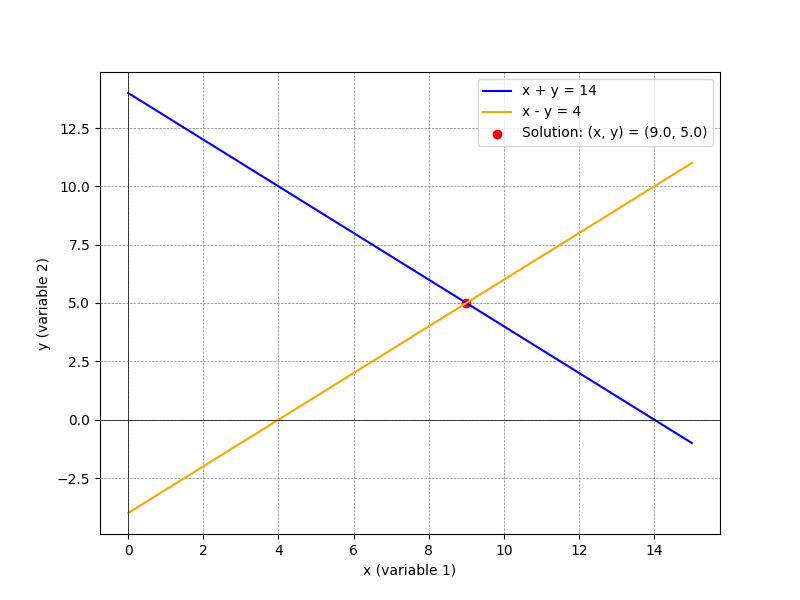
\includegraphics[width=\columnwidth]{figs/fig.png}
\end{figure}
\end{enumerate}
\end{document}
